\chapter{实验}
\label{cha:experiment}
在本章中,我们分别介绍对某一目标的情感分析(Aspect-Term Sentiment Analysis or Target-oriented Sentiment Analysis)和新闻驱动的股票预测的实验设置及实验结果。

\section{对某一目标的情感分析}
在本小节,我们介绍对某一目标的情感分析(Aspect-Term Sentiment Analysis or Target-oriented Sentiment Analysis)的实验。这里,我们使用的是基于transformer和多尺度卷积的模型。
\subsection{实验设置}
我们在餐厅(Restaurant)、笔记本电脑(Laptop)、推特(Twitter)三个公开数据集上进行了实验。这三个数据集均在第~\ref{cha:data}章中有所介绍。我们沿用了之前工作中数据预处理的方法~\cite{Xin2018Transformation,Tang2015Effective},我们除去了一些冲突的标签,所有单词均转化为小写,不去除任何的停止词、符号、数字。我们使用nltk\footnote{http://www.nltk.org/}工具提供的分词工具对全部的句子进行分词。所有的句子都使用“PAD”字符补齐成最大长度。

我们使用准确率和macro-averaged F1 score作为评价指标。对每一类来说,精确率$P=\frac{TP}{TP+FN}$,召回率$R=\frac{TP}{TP+FP}$,F1 score由$\frac{2PR}{P+R}$求得。Macro-averaged F1 score是所有类别的F1 score的均值~\cite{Tang2015Effective}。

我们与下列模型进行了对比:
\begin{itemize}
    \item Majority把训练集中出现频率最高的类别作为预测类别;
    \item SVM是支持向量机模型,它使用的是人为构建的n-gram特征、解析特征和语义特征~\cite{kiritchenko2014nrc-canada-2014};
    \item AE-LSTM是一个将目标和句子拼接起来作为输入的LSTM模型;
    \item ATAE-LSTM对AE-LSTM进行了扩展,利用attention机制选取最重要的单词~\cite{wang2016attention-based};
    \item IAN利用交互式地方式,分别使用attention方法计算句子和目标的表示~\cite{ma2017interactive};
    \item BILSTM-ATT-G使用控制门来控制目标左边、右边部分的重要性~\cite{liu2017attention};
    \item GCAE使用卷积神经网络和控制门,得到了更高的准确率,更容易并行化~\cite{xue2018aspect};
    \item {Memnet}将词向量当作记忆单元,使用多层attention方法来得到最终表示,为克服attention机制不能获取时序信息的缺点,它还使用了位置权重~\cite{tang2016aspect};
    \item RAM对Memnet做出了改进,它使用双向LSTM的结果作为记忆单元,使用GRU来生成下一层的表示,同时使用了与Memnet不同的位置权重~\cite{Al2017Deep};
    \item TNet提出生成与目标相关的句子表示,同时结合上下文信息。\cite{Xin2018Transformation}.
\end{itemize}
我们使用pytorch\footnote{https://pytorch.org}框架实现了这些模型中除IAN之外的模型,并使它们的实验结果尽可能地与原论文相似。每个模型都是独立训练的。我们使用的是GloVe~\cite{pennington2014glove}词向量来初始化我们的词向量,并在训练的过程中调整词向量的值。句子的最大长度设为30。
在我们的模型中,我们使用的模型参数设置与OpenAI GPT~\cite{radford2018improving}一致。具体地,transformer的层数是12,多头attention的head数是12,词向量的维度设为768,中间层的维度设为了3072。我们首先加载OpenAI GPT~\cite{radford2018improving}的预训练参数,然后与后续结构一起进行调优。我们使用了五个不同的卷积核,卷积核大小从1到5。卷积的输出通道数设为100。我们使用Adam~\cite{kingma2014adam}优化器,学习率设为6.25e-5。模型在20轮训练内就得到了最好的效果。
\subsection{实验结果}

\begin{table}[ht]
    \centering
    \caption[对某一目标的情感分析实验结果]{对某一目标的情感分析实验结果(\%),带“*”的实验结果是从原文中获取的}
    \label{tab:result}
    \begin{tabular}{lcccccc}
    \hlinewd{1.5pt}
    \multirow{2}{*}{Models} & \multicolumn{2}{l}{Restaurant} & \multicolumn{2}{l}{Laptop} & \multicolumn{2}{l}{Twitter} \\ \cline{2-7} 
                            & ACC       & Macro-F1      & ACC     & Macro-F1    & ACC     & Macro-F1     \\ \hline
    Majority                &65.00           &-              &53.45         &-            &50.00         &22.22         \\
    SVM                     &80.89           &-              &72.10         &-            &63.40         &63.30         \\ 
    LSTM                    &76.70           &63.57          &69.28         &63.30        &66.04         &63.46         \\
    ATAE-LSTM               &77.23           &63.73          &69.44         &63.46        &71.24         &69.19         \\
    IAN                     &78.60$^*$       &-              &72.10$^*$     &-            &-             &-             \\
    BILSTM-ATT-G            &79.20           &67.07          &71.32         &64.88        &71.68         &70.37         \\
    GCAE                    &78.12           &62.50          &70.38         &64.02        &72.40         &70.89         \\
    MemNet                  &77.86           &64.47          &68.18         &62.46        &69.80         &66.86         \\
    RAM                     &78.30           &65.42          &71.63         &66.73        &71.24         &68.75         \\
    TNet                    &78.39           &65.37          &73.98         &68.64        &72.11         &70.01         \\ \hline
    Ours                    &84.91           &76.40          &78.37         &74.05        &74.86         &73.63         \\ \hlinewd{1.5pt}
    \end{tabular}
    \end{table}
表~\ref{tab:result}显示了对某一目标的情感分析的实验结果。我们的模型在Restaurant、Laptop、Twitter数据集上均取得了最佳的实验结果。我们在Restaurant数据集上取得了84.91\%的准确率(提升6.52\%),在Laptop数据集上取得了78.37\%的准确率(提升4.39\%),在推特数据集上取得了74.86\%的准确率(提升2.75\%)。

在所有的神经网络模型中,LSTM模型效果最差。ATAE-LSTM考虑到了目标并使用了attention方法,效果有所提升。IAN使用了句子对目标的attention和目标对句子的attention,更进一步提升了实验效果。BILSTM-ATT-G和RAM在Restaurant和Laptop上的实验效果较好,但在Twitter数据集上效果提升并没有那么大,可见LSTM不擅长处理Twitter数据中大量的口语化文本。TNet使用了CNN和LSTM,并在三个数据集上都取得了不错的效果。

不同于这些模型,我们的模型使用transformer提取句子特征,更易于处理长期依赖关系,易于并行。我们的模型利用多尺度卷积,从不同粒度提取特征。我们的模型在三个数据集上的实验效果比其他几个模型要好。
\subsection{预训练}
为了证明transformer预训练的效果,我们进行了对比实验:一组使用预训练的transformer参数,另一组完全随机初始化参数,并从头开始进行训练。
\begin{table}[h]
    \centering
    \caption{预训练的作用}
    \label{tab:pretrain}
    \begin{tabular}{lcccc}
         \hlinewd{1.5pt}
     \multirow{2}{*}{\textbf{Models}} & \multicolumn{2}{c}{Restaurant} & \multicolumn{2}{c}{Laptop} \\
     \cline{2-5}
                                      & ACC & Marco-F1 & ACC & Marco-F1 \\
    \hline
         w/o pre-training & $69.20$ & $48.16$ & $64.89$ & $59.25$ \\
         w/ pre-training & $84.91$ & $76.40$ & $78.37$ & $74.05$ \\
    \hlinewd{1.5pt}
    \end{tabular}
\end{table}
表~\ref{tab:pretrain}显示了对比实验的实验结果。当不使用预训练的参数时,实验效果大大下降。在预训练的过程中,深层transformer模型通过前几个单词去预测下一个单词;在这一过程中,模型学习到了语言的表示方式,并将这些知识迁移到后续的任务当中。

\subsection{多尺度卷积}
为证明多尺度卷积的重要性,我们将模型中的多尺度卷积去掉,对比了简化后的模型与完整模型的实验效果。
\begin{table}[h]
    \centering
    \caption{多尺度卷积的作用}
    \label{tab:cnn}
    \begin{tabular}{lcccc}
         \hlinewd{1.5pt}
     \multirow{2}{*}{\textbf{Models}} & \multicolumn{2}{c}{Restaurant} & \multicolumn{2}{c}{Laptop} \\
     \cline{2-5}
                                      & ACC & Marco-F1 & ACC & Marco-F1 \\
    \hline
         w/o cnn & $83.39$ & $74.40$ & $77.43$ & $72.42$ \\
         w/ cnn & $84.91$ & $76.40$ & $78.37$ & $74.05$ \\
    \hlinewd{1.5pt}
    \end{tabular}
\end{table}
表~\ref{tab:cnn}显示了对比实验的结果。多尺度卷积能够利用全部单词的表示信息,提取不同长度的短语的表示,并选取最为重要的信息。多尺度卷积将Restaurant数据集上的准确率提升约1.52\%,将Laptop数据集上的准确率提升约0.94\%。
\subsection{样例分析}
\begin{table}[ht]
    \centering
    \caption[结果示例]{结果示例,输入目标用中括号标记,正确输出标签以标的形式给出}
    \label{tab:case}
    \begin{tabular}{m{7cm}>{\centering\arraybackslash}m{1cm}>{\centering\arraybackslash}m{1cm}>{\centering\arraybackslash}m{1cm}}
    \hlinewd{1.5pt}
    Sentence & ATAE-LSTM & GCAE & Ours  \\ \hline
    {[}Coffee{]}$_P$ is a better deal than overpriced sandwiches.      
    & $P$  & $O$\textsuperscript{\xmark} & $P$ \\ \hline
    But make sure you have enough room on your credit card as the {[}bill{]}$_P$ will leave a big dent in your wallet. 
    & $P$ & $O$\textsuperscript{\xmark} & $P$ \\ \hline
    Aww, it 's okay... You have a {[}PSP{]}$_P$. :D That 's good already.
    & $O$\textsuperscript{\xmark} & $P$ & $P$ \\ \hline
    I hate my {[}iPod{]}$_N$! It's dead! dead dead dead! ! ! Someone wanna fix it for me?
    & $O$\textsuperscript{\xmark} & $N$ & $N$ \\ \hline
    I have never had a bad {[}meal{]}$_P$ (or bad service) at pigalle.
    & $N$\textsuperscript{\xmark} & $N$\textsuperscript{\xmark} & $P$ \\ \hline
    The {[}staff{]}$_N$ should be a bit more friendly. 
    & $P$\textsuperscript{\xmark} & $P$\textsuperscript{\xmark} & $N$ \\ \hline
    It's a basic pizza joint, not much to look at, but the {[}pizza{]}$_P$ is what I go for.
    & $N$\textsuperscript{\xmark} & $O$\textsuperscript{\xmark} & $P$ \\ \hline
    \hlinewd{1.5pt}
    \end{tabular}
\end{table}
表~\ref{tab:case}显示了一些预测的例子。输入目标用中括号标记,正确输出标签以下标的形式给出。其中$P$、$N$、$O$分别表示积极、消极和中立。比如,在第一个句子中,对“coffee”的情感极性是积极的。我们的模型比ATAE-LSTM和GCAE的预测结果要好。前两行中,句子的句式比较正式,LSTM的模型更擅长解决此类问题。后两行中,包含像“Aww, it's okay...”和“It's dead dead dead!!”这样的表达,句子比较口语化,句子结构比较零散,CNN更擅长解决此类问题。Transformer的模型经过了大规模语料库的预训练,在处理这两种情况时都有不错的表现。另外,我们的模型具备一定的推理和比较的能力,第五行中,“never”和“bad”的双重否定得到了积极的预测结果;第六行中,“should be”是本应该的意思,暗含员工的服务态度并没有那么好。最后一行,表示情感的词是“what I go for”,因为使用了多尺度卷积,我们的模型可以提取到短语的信息。
\section{新闻驱动的股票预测}
在本小节中,我们介绍新闻驱动的股票预测相关实验。我们使用的是基于注意力机制的多股票关系模型(Multi-Stock Relation Model using Attention Mechanism)。
\subsection{实验设置}
我们在前面提到的senti-stock数据集上进行实验。所有单词都转化为小写,不移除任何停止词、符号或数字。我们使用nltk\footnote{http://www.nltk.org/}工具提供的分词工具对全部的句子进行分词。所有句子用"PAD"符号补齐到最大长度。我们以准确率和F1平均值为主要的评价指标。对每一类而言,精确率$P=\frac{TP}{TP+FN}$,召回率$R=\frac{TP}{TP+FP}$,F1值由$\frac{2PR}{P+R}$求得。其中,$TP$、$TN$、$FN$、$FP$分别表示真正例、真负例、假负例、假正例的个数。最终的F1平均值是各个类的F1值的均值。相比于准确率,F1值更能评价在不均衡数据集下预测结果的好坏。

在前面提到了基于方面的情感分析模型中,有一些模型要求目标必须出现在句子当中,或目标不止包含有一个单词,因此不能应用到新闻驱动的股票预测这一场景当中。因此,我们的模型只与下列模型进行了对比:
\begin{itemize}
    \item Majority将训练集中大多数的标签作为测试集的预测标签。
    \item LSTM利用简单的LSTM来处理新闻句子信息,不考虑股票的相关信息。
    \item ATAE-LSTM在LSTM的基础上,引入了attention机制,结合了股票信息和新闻句子信息。
    \item GCAE使用CNN来处理新闻句子,通过CNN计算得到了gate来调整预测的结果。
\end{itemize}
我们使用pytorch\footnote{https://pytorch.org}复现了上述模型。每个模型都是独立训练的。句子最大长度设为30。每个模型都使用GloVe\cite{pennington2014glove}预训练的词向来初始化词向量,词向量的维度是300。CNN的卷积核大小从3到5,卷积的输出通道数设为100。我们使用AdaGrad~\cite{duchi2011adaptive}优化器,学习率设为0.01。模型的实现是开源的\footnote{https://www.github.com/Cppowboy/icann2019}。
\subsection{实验结果}
\begin{table}[ht]
    \centering
    \caption{senti-stock数据集上的实验结果}
    \label{tab:mainresult}
    \begin{tabular}{lcccccc}
    \hlinewd{1.5pt}
    \multirow{2}{*}{Models} & \multicolumn{2}{c}{Short}         & \multicolumn{2}{c}{Middle}        & \multicolumn{2}{c}{Long}                                \\ \cline{2-7} 
                            & Accuracy        & Macro-F1        & Accuracy        & Macro-F1        & Accuracy                   & Macro-F1                   \\ \hline
    Majority                & 0.5710          & 0.2423          & 0.3832          & 0.1847          & 0.4789                     & 0.2158                     \\
    LSTM                    & 0.6316          & 0.5542          & 0.5655          & 0.5594          & 0.6162                     & 0.5641                     \\
    ATAE-LSTM               & 0.6401          & 0.5688          & 0.5687          & 0.5663          & 0.6241                     & 0.5791                     \\
    GCAE                    & 0.6828          & 0.6072          & 0.6097          & 0.6047          & 0.6630                     & 0.6161                     \\
    MSRMAM                    & \textbf{0.6920} & \textbf{0.6198} & \textbf{0.6273} & \textbf{0.6237} & \textbf{0.6826}            & \textbf{0.6387}            \\ \hlinewd{1.5pt}
    \end{tabular}
\end{table}
表~\ref{tab:mainresult}显示了在senti-stock数据集上的主要实验结果。LSTM在所有神经网络模型中效果最差,因为它只考虑了新闻句子的信息,没有考虑股票的相关信息。ATAE-LSTM引入了attention机制,考虑了股票相关信息,使得它相比LSTM有所提升。GCAE使用了CNN来处理新闻标题这种比较简洁的文本,取得了更好的效果。我们所提出的模型在三种不同的时间间隔上的预测取得了不错的效果。
\begin{figure}[H]
    \centering 
    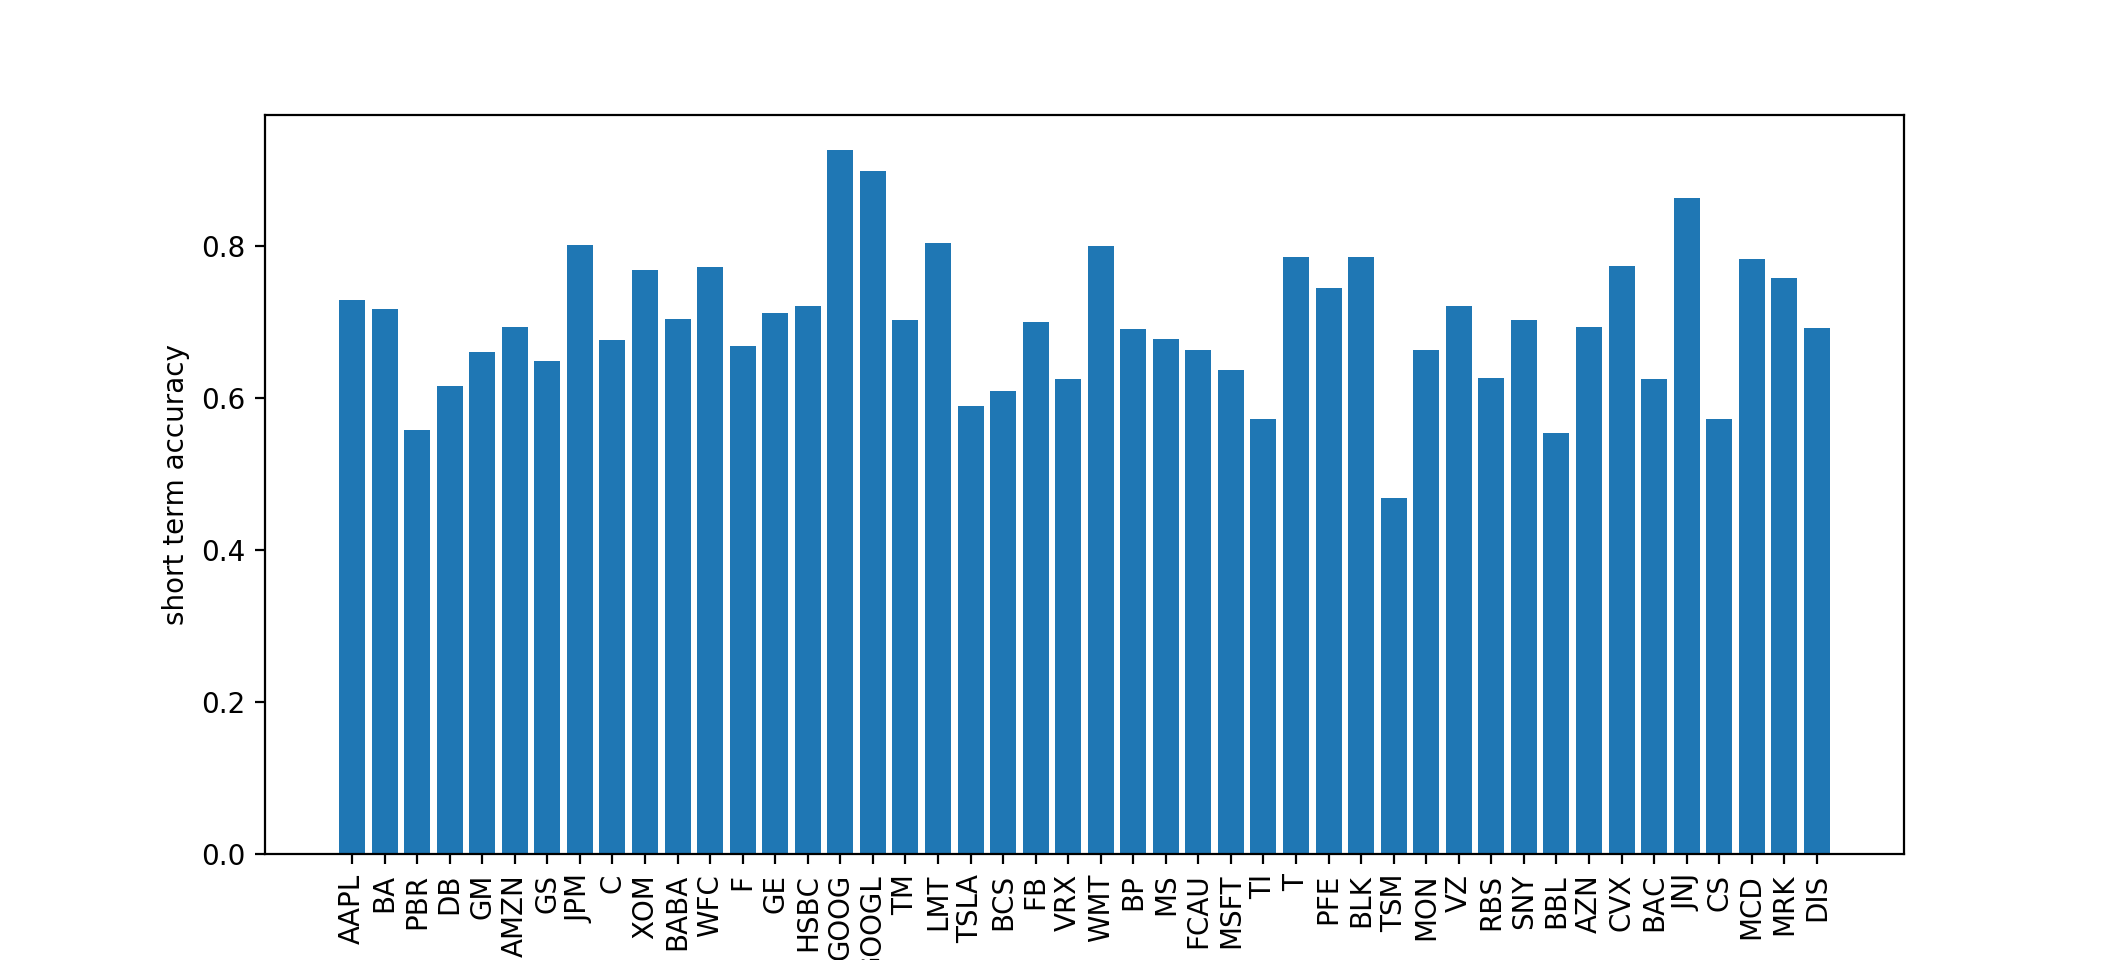
\includegraphics[width=\linewidth]{short-acc.png}
    \caption{各股票短期预测准确率}
    \label{fig:short-acc}
\end{figure}
\begin{figure}[H]
    \centering 
    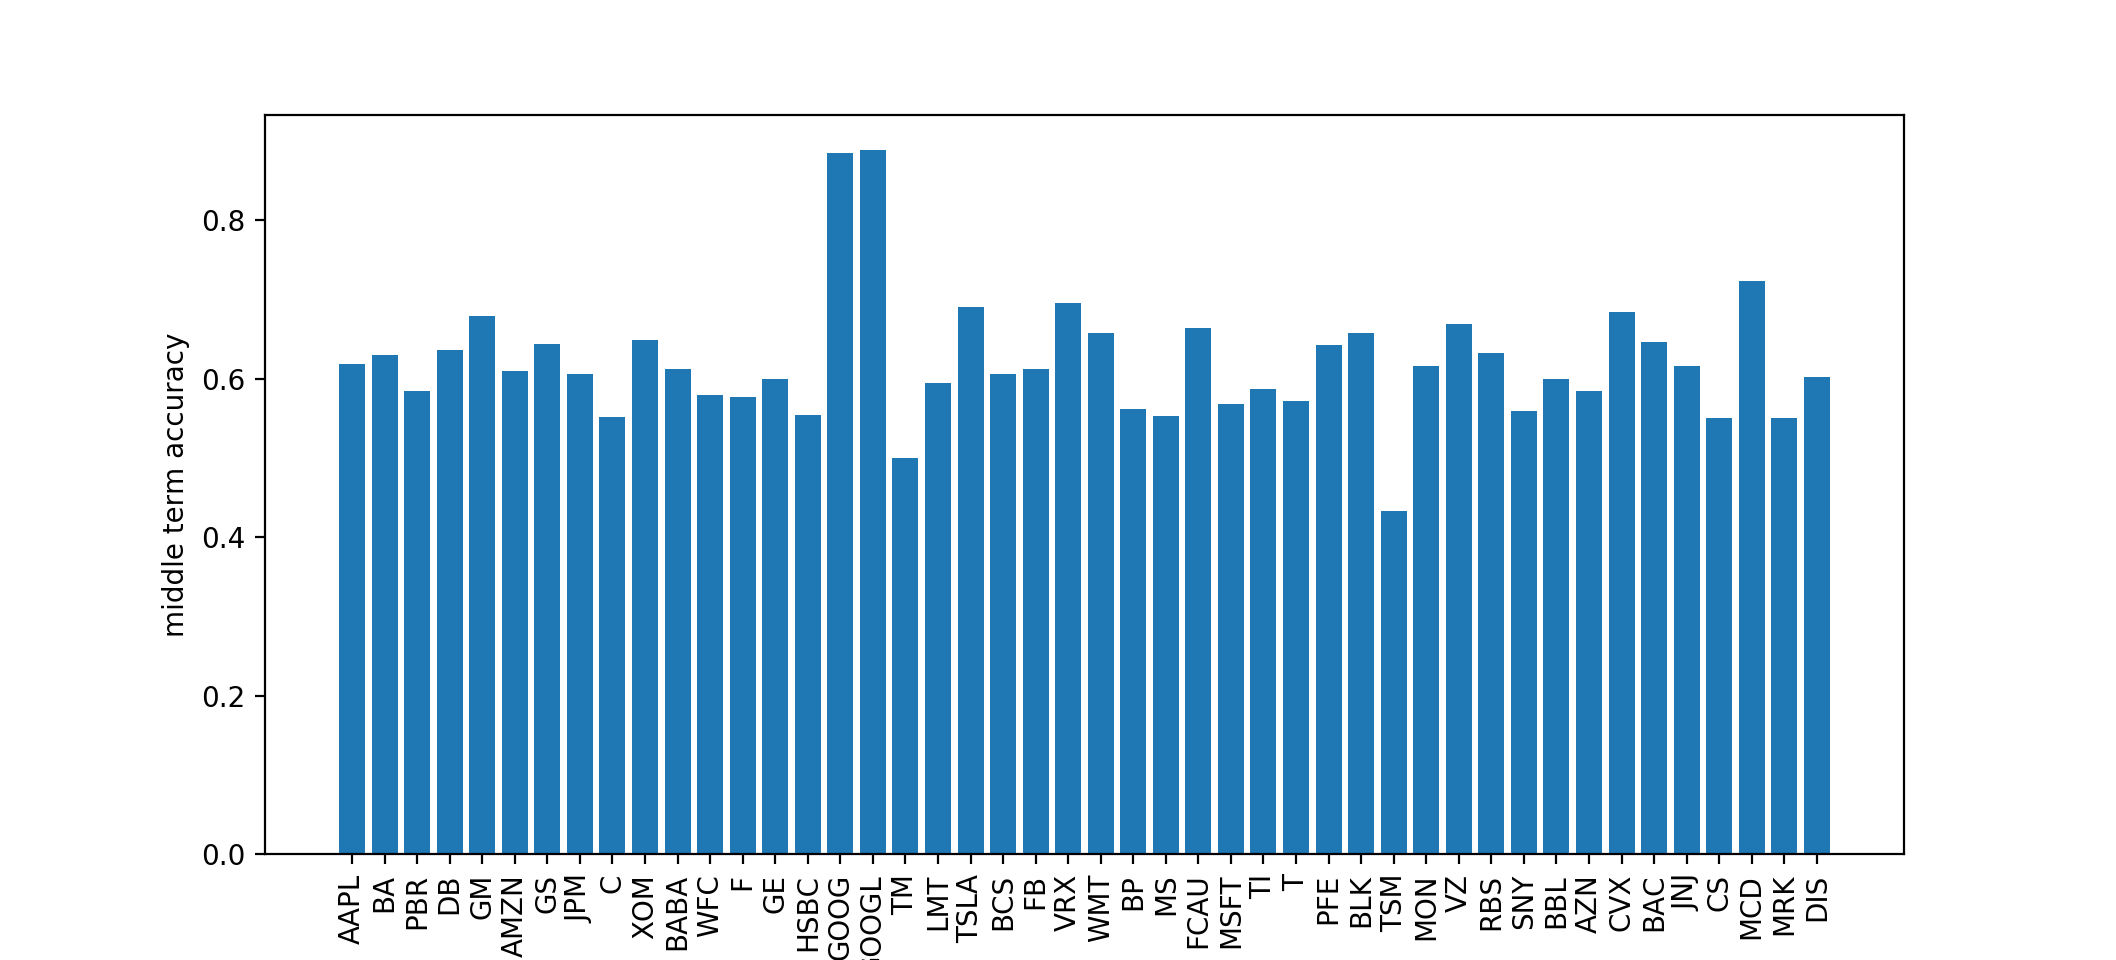
\includegraphics[width=\linewidth]{middle-acc.png}
    \caption{各股票中期预测准确率}
    \label{fig:middle-acc}
\end{figure}
\begin{figure}[H]
    \centering 
    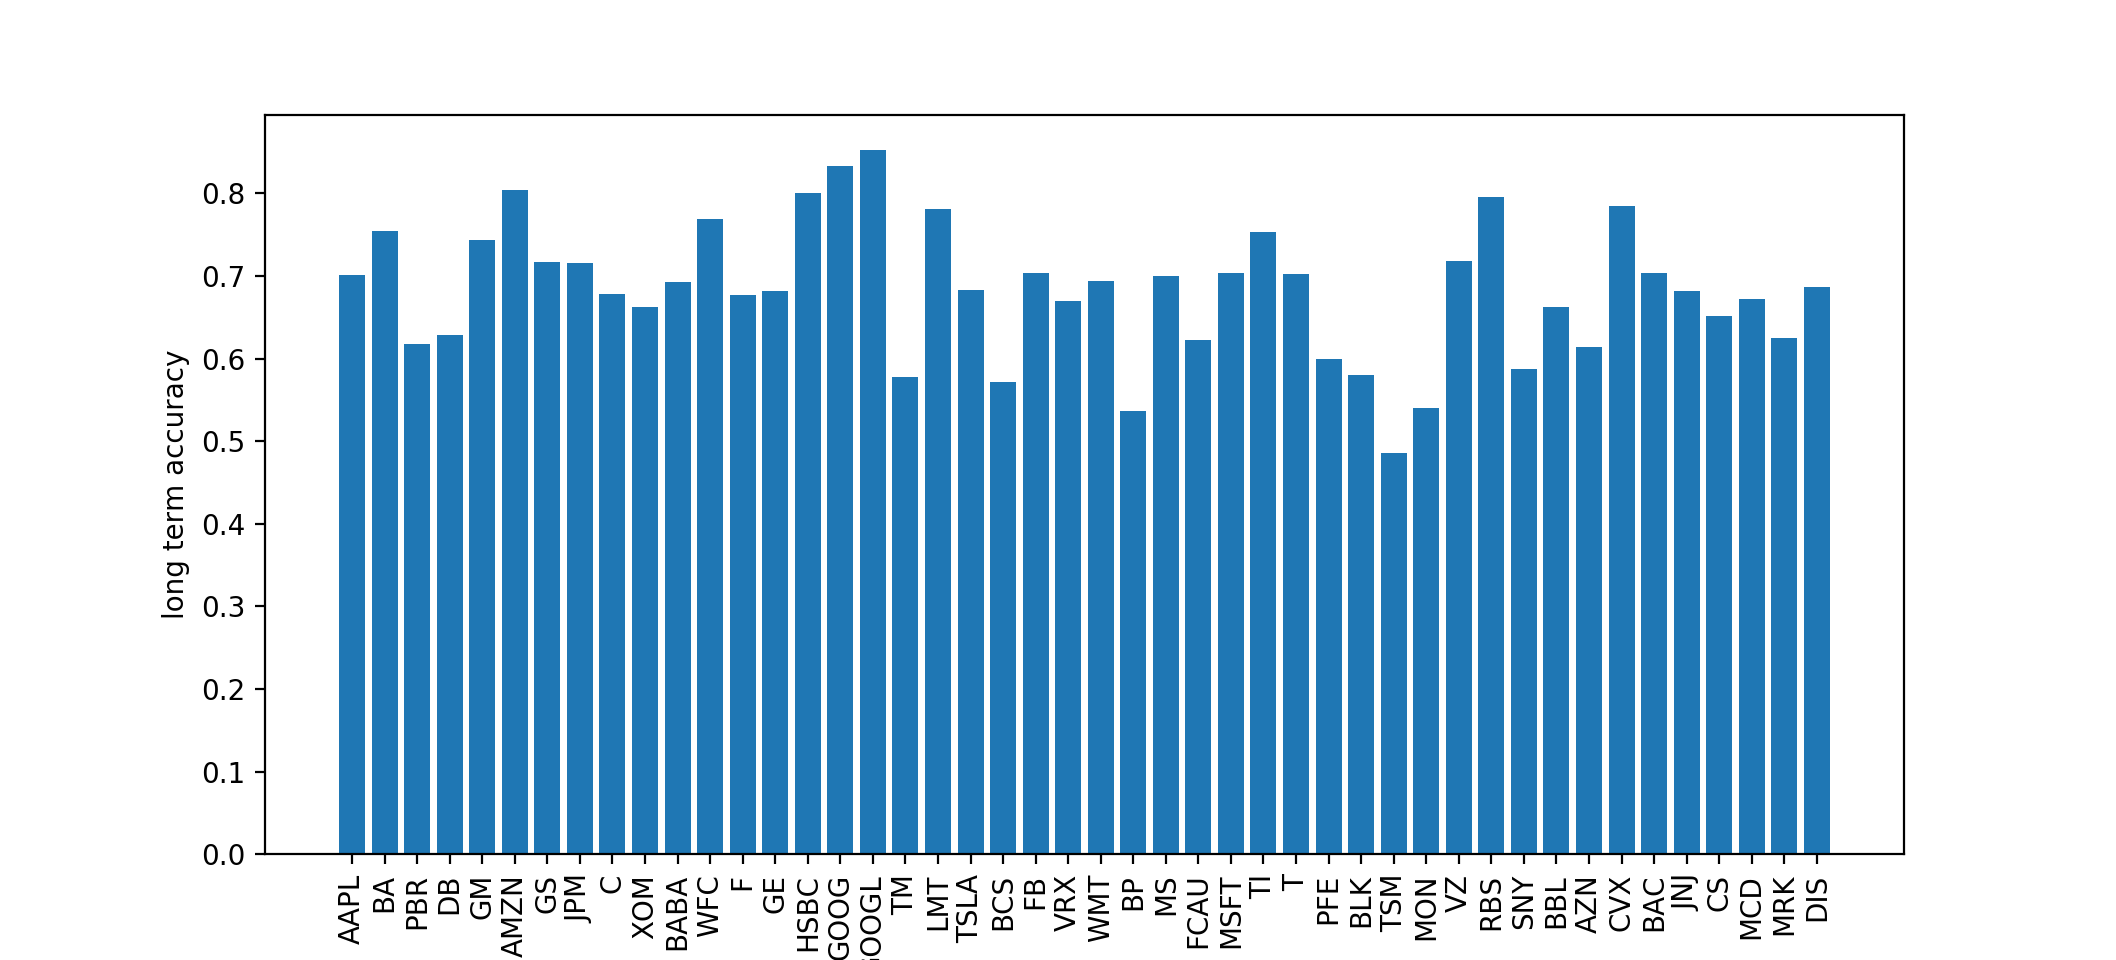
\includegraphics[width=\linewidth]{long-acc.png}
    \caption{各股票长期预测准确率}
    \label{fig:long-acc}
\end{figure}
图\ref{fig:short-acc}、图\ref{fig:middle-acc}、图\ref{fig:long-acc}分别显示了各支股票的短期、中期、长期的预测准确率。短期预测和长期预测的准确率明显比中期预测要高,大部分股票的短期和长期预测准确率均超过了百分之五十。而中期预测的准确率相对较低,大部分股票的中期预测准确率超过了百分之四十。谷歌(GOOG)在短期、中期和长期的预测准确率均超过了百分之八十,说明谷歌的股票价格与其相关新闻关系非常密切。
\subsection{模型简化实验}

\begin{table}[ht]
    \centering
    \caption{模型简化实验结果}
    \label{tab:ablation}
    \begin{tabular}{lcccccc}
    \hlinewd{1.5pt}
    \multirow{2}{*}{Models} & \multicolumn{2}{c}{Short}         & \multicolumn{2}{c}{Middle}        & \multicolumn{2}{c}{Long}                                \\ \cline{2-7} 
                            & Accuracy        & Macro-F1        & Accuracy        & Macro-F1        & Accuracy                   & Macro-F1                   \\ \hline
    CNN                     & 0.6498          & 0.5786          & 0.5813          & 0.5761          & \multicolumn{1}{c}{0.6490} & \multicolumn{1}{c}{0.5961} \\
    MCNN                    & 0.6616          & 0.5852          & 0.5920          & 0.5871          & \multicolumn{1}{c}{0.6531} & \multicolumn{1}{c}{0.6005} \\
    MCSC                    & \textbf{0.6955} & \textbf{0.6208} & 0.6236          & 0.6205          & 0.6765                            & 0.6275                     \\ 
    MSRMAM                    & 0.6920          & 0.6198          & \textbf{0.6273} & \textbf{0.6237} & \textbf{0.6826}                   & \textbf{0.6387}            \\ \hlinewd{1.5pt}
    \end{tabular}
\end{table}
为了证明MSRMAM模型各个部分的有效性,我们进行了模型简化实验。CNN是一个基本的卷积神经网络模型,它只考虑新闻句子的输入,不考虑股票的信息。MCNN使用了多尺度卷积,可以提取不同长度的短语的信息。MCSC使用了股票系数,股票系数引入了股票相关信息。MSRMAM是我们的完整模型,它使用了attention机制,学习股票之间的相关关系。从表~\ref{tab:ablation}可以看到,多尺度卷积和股票系数都可以明显地提升模型的性能。股票关系模型对中期和长期的预测有更大的作用。一种可能的解释是,股票关系模型反映了股票之间的相互关系,这些股票关系与基本面分析更加相关,在中长期的股票价格变动中能展现较大的作用;但在短期预测中,股票价格变化时效性更强,股票关系影响较小。

\subsection{样例分析}

\begin{table}
    \centering  
    \caption{新闻驱动的股票预测样例分析}
    \label{tab:stockcase}
    \begin{tabular}{m{7cm}lm{1cm}m{1cm}m{1.8cm}}
        \hlinewd{1.5pt}
        news title & stock & ATAE-LSTM & GCAE & MSRMAM \\ \hline 
        Tesla delivers quarterly record of 25000 vehicles in first quarter & TSLA\textsubscript{+1} & +1\textsuperscript{\cmark} & -1\textsuperscript{\xmark} & +1\textsuperscript{\cmark} \\  \hline
        Taiwan stocks hit over 18-mth highs TSMC up ahead of Q4 result & TSM\textsubscript{+1} & +1\textsuperscript{\cmark} & 0\textsuperscript{\xmark} & +1\textsuperscript{\cmark} \\ \hline 
        %        Morgan Stanley's profit doubles on bond-trading surge & MS\textsubscript{+1} & -1\textsuperscript{\xmark} & +1\textsuperscript{\cmark} & +1\textsuperscript{\cmark} \\ \hline
        AT\&T to offer hulu to customers this year. & T\textsubscript{+1} & 0\textsuperscript{\xmark} & +1\textsuperscript{\cmark} & +1\textsuperscript{\cmark} \\ \hline
        Consumer reports says Tesla misunderstands 'positive' Model 3 rating & TSLA\textsubscript{-1} & +1\textsuperscript{\xmark} & -1\textsuperscript{\cmark} & -1\textsuperscript{\cmark} \\ \hline
        % Amazon-Apple TV deal shows tough road to cooperation for tech rivals & AMZN\textsubscript{-1} & 0\textsuperscript{\xmark} & -1\textsuperscript{\cmark} & -1\textsuperscript{\cmark} \\ \hline 
        % Apple Google reach new deal with workers xin U.S. lawsuit over hiring & AAPL\textsubscript{+1} & 0\textsuperscript{\xmark} & +1\textsuperscript{\cmark} & +1\textsuperscript{\cmark} \\ \hline
        %        Amazon offers prime discount for U.S. customers on government aid & AMZN\textsubscript{-1} & 0\textsuperscript{\xmark} & 0\textsuperscript{\xmark} & -1\textsuperscript{\cmark} \\ \hline
        % Wal-Mart takes on amazon 's 'prime day ' with online sale & WMT\textsubscript{1} & +1\textsuperscript{\xmark} & +1\textsuperscript{\xmark} & +1\textsuperscript{\xmark} \\ \hline  
        Tesla has recalled 53 000 of its model s model x cars & TSLA\textsubscript{+1} & -1\textsuperscript{\xmark} & -1\textsuperscript{\xmark} & -1\textsuperscript{\xmark} \\ \hlinewd{1.5pt}
    \end{tabular}
\end{table}
为了进一步分析MSRMAM模型的特点,我们在表\ref{tab:stockcase}中展示了新闻驱动的股票预测的样例,正确预测值以下标的形式给出。我们比较了以ATAE-LSTM为代表的LSTM模型和以GCAE为代表了CNN模型,以及我们所提出的股票关系模型。在前两行所展示的例子中,句子都是比较正式,更高的销量或营收可以预测股票价格上涨,LSTM更擅长处理此类问题。在第三行的例子中,因为标题的简洁性,标题与普通句子的语法并不完全一致,CNN能够很好地处理此类问题。第四行中,“misunderstands 'positive' rating”,LSTM误将“positive”识别为积极的消息,CNN模型可以将误解与积极联系成一个短语。另外,在最后一行的例子中,模型预测消息是消极的,从人的主观观察来看,这一结果是正确的,但是,它与股票实际的涨跌不同。我们之前假设股票价格的涨跌仅与前一天、周、月的相关新闻有关,而忽视了其他因素。然而在现实当中,其他因素也发挥着重要作用,新闻并不是决定股票涨跌的唯一因素。为了进一步提升股票预测的准确率,我们可以考虑补充股票历史价格、技术指标等其他信息,这也是后续研究的方向之一。
% \subsection{市场模拟}
% 为了进一步验证我们的模型效果,我们进行了市场模拟实验。我们采用了这样的交易策略\cite{lavrenko2000mining}:我们每天进行一次预测,如果预测某支股票的价格在下一个时间段(天、周、月)内会上涨,则买入价值一万美金的这支股票,如果在下一个时间段内(天、周、月),股票价格上涨超过百分之一,则将其卖出,否则,在下一天、周或月后,将股票卖出;如果预测某支股票价格在下一个时间段(天、周、月)内会下跌,则买空一万美金的这支股票,如果在下一个时间段内(天、周、月),股票价格下跌超过百分之一,则将其卖空,否则,在下一天、周或月后,将股票卖空。我们将初始资金设为三万美金,并利用历史数据进行训练和模拟。我们将购买标普500指数并持有作为基准策略,无风险收益定为百分之三。

% \subsection{策略风险评价指标}

% 策略的风险指标能够从各个维度对策略有客观、全面的评估。本文中,我们使用了以下风险评价指标。
% \subsubsection{年化收益率}
% 年化收益率(Annualized Returns)表示投资一年的预期收益率。
% \begin{equation}
%     p_r=(\frac{p_{end}}{p_{start}})^{\frac{250}{n}}-1
% \end{equation}
% 其中,$p_{end}$是策略最终总资产,$p_{start}$是策略初始总资产,$n$是交易日数量。
% \subsubsection{基准年化收益率}
% 基准年化收益率(Benchmark Returns)表示参考标准年化收益率。
% \begin{equation}
%     B_r=(\frac{B_{end}}{B_{start}})^{\frac{250}{n}}-1
% \end{equation}
% 其中,$B_{end}$是基准最终值,$B_{start}$是基准初始值,$n$是交易日数量。
% \subsubsection{贝塔}
% 贝塔(Beta)表示投资的系统性风险,反映了策略对大盘变化的敏感性。例如,一个策略的Beta为1.3,则大盘涨1\%的时候,策略可能涨1.3\%,反之亦然;如果一个策略的Beta为-1.3,说明大盘涨1\%的时候,策略可能跌1.3\%,反之亦然。
% \begin{equation}
%     \beta=\frac{Cov(p_n,B_n)}{\sigma^2_B}
% \end{equation}
% 其中,$p_n$是策略每日收益率,$B_n$是基准每日收益率,$\sigma^2_B$基准每日收益方差,$Cov(p_n,B_n)$是策略和基准每日收益的协方差。
% \subsubsection{阿尔法}
% 投资中面临着系统性风险(即Beta)和非系统性风险(即Alpha)。Alpha是投资者获得与市场波动无关的回报,一般用来度量投资者的投资技艺。例如,投资者获得了12\%的回报,其基准获得了10\%的回报,那么Alpha或者价值增值的部分就是2\%。
% \begin{equation}
%     \alpha=p_r-r_f-\beta(B_r-r_f)
% \end{equation}
% 其中,$p_r$是策略年化收益率,$r_f$是无风险收益率,$B_r$是基准年化收益率。当Alpha大于零时,说明策略相对于风险,获得了超额收益;当Alpha等于零时,说明策略相对于风险,获得了适当收益;当Alpha小于零时,说明策略相对于风险,获得了较少收益。
% \subsubsection{收益波动率}
% 收益波动率(Volatility)用来测量资产的风险性,波动越大代表策略风险越高。
% \begin{equation}
%     \sigma_p=\sqrt{\frac{250}{n}\sum_{t=1}^{n}(p_t-\overline{p_t})^2}
% \end{equation}
% 其中,$n$是交易日数量,$p_t$是策略每日收益率,$\overline{p_t}=\frac{1}{n}\sum_{t=1}^{n}p_t$策略每日平均收益率。
% \subsubsection{夏普比率}
% 夏普比率(Sharpe Ratio)表示每承受一单位总风险,会产生多少的超额报酬,可以同时对策略的收益与风险进行综合考虑。
% \begin{equation}
%     SharpRatio=\frac{p_r-r_f}{\sigma_p}
% \end{equation}
% 其中,$p_r$是策略年化收益率,$r_f$是无风险收益率,$\sigma_p$是策略收益率波动率
% \subsubsection{信息比率}
% 信息比率(Information Ratio)用来衡量单位超额风险带来的超额收益。信息比率越大,说明该策略单位跟踪误差所获得的超额收益越高,因此,信息比率较大的策略的表现要优于信息比率较小的策略。合理的投资目标应该是在承担适度风险下,尽可能追求高信息比率。
% \begin{equation}
%     InformationRatio=\frac{p_r-B_r}{\sigma_t}
% \end{equation}
% 其中,$p_r$是策略年化收益率,$B_r$是基准年化收益率,$\sigma_t$是策略与基准每日收益差值的年化标准差。
% \subsubsection{最大回辙}
% 最大回撤(Max Drawdown)描述策略可能出现的最糟糕的情况。
% \begin{equation}
%     MaxDrawDown_t=max(1-\frac{P_j}{P_i})
% \end{equation}
% $MaxDrawDown_t$为$t$日的最大回撤,$P_i$和$P_j$分别为$i$日和$j$日的策略总资产,其中$t\ge j>i$。

\subsection{风险提示}
利用MSRMAM模型进行新闻驱动的股票预测是对历史经验的总结,存在失效的可能。股市有风险,投资须谨慎。